\begin{frame}
	\centering
	{\Huge Introdução}
\end{frame}

\section{Introdução}\label{sec:introducao}

% ----------------- SLIDE 1 --------------------------------

\begin{frame}{Introdução}
	\begin{block}{}
		\begin{itemize}
			\item Avanço dos computadores e redes de comunicação;
			\item Computadores pessoais ---> Servidores \textit{web};
			\item Acessíveis no mundo todo;
			\item Servidores HTTP.
		\end{itemize}
	\end{block} \pause
	\begin{block}{}
		\begin{itemize}
			\item Conteúdo dinâmico;
			\item Ambientes chegando ao limite;
			\item Fragilidades expostas;
			\item Falta desempenho.
		\end{itemize}
	\end{block}
\end{frame}
% ----------------- SLIDE 2 --------------------------------
\begin{frame}{Escalabilidade}
	\begin{block}{Escalabilidade}
		``Escalabilidade é um atributo desejável de 
		uma rede, sistema ou processo.'' (BONDI, 2000).
		\begin{itemize}
			\item Acomodar uma quantidade sempre maior de elementos ou objetos; 
			\pause
			\item Processar quantidade crescente de trabalho; \pause
			\item Suscetível a ampliação;
		\end{itemize}
	\end{block}
\end{frame}
% ----------------- SLIDE 3 --------------------------------
\begin{frame}{Escalabilidade}
	\begin{block}{Escalabilidade}
		Quando se diz que um sistema não é escalável ou que não escala:
		\begin{itemize}
			\item Custo adicional é excessivo; \pause
			\item Tempo de resposta; \pause
			\item Processamento (processador); \pause
			\item Espaço; \pause
			\item Memória; \pause
			\item Dinheiro.
		\end{itemize}
	\end{block}
\end{frame}
% ----------------- SLIDE 4 --------------------------------
\begin{frame}{Escalabilidade}
	\begin{block}{Escalabilidade}
		\begin{itemize}
			\item É crucial para o sucesso à longo prazo de um sistema; \pause
			\item Pode ser comprometida por ações repetidas de forma frequente; 
			\pause
			\item Algoritmos que levem a \textit{deadlock}; \pause
			\item Escalonamento de recursos ruim.
		\end{itemize}
	\end{block}
\end{frame}
% ----------------- SLIDE 5 --------------------------------
\begin{frame}{SIGA}
	\begin{block}{SIGA}
		\begin{itemize}
			\item Adquirido em 2007 da UFJF; \pause
			\item PHP e Miolo; \pause
			\item Apache HTTP \textit{Server}.
		\end{itemize}
	\end{block} \pause
	\begin{block}{Apache}
		\begin{itemize}
			\item Desenvolvido desde 1.995;
			\item Mais utilizado desde então;
			\item Aproximadamente 37\% dos sítios no mundo.
		\end{itemize}
	\end{block}
\end{frame}
% ----------------- SLIDE 6 --------------------------------
\begin{frame}{Utilização dos Servidores \textit{Web}}
	\begin{figure}
		\centering
		\caption{Utilização de Servidores \textit{web} no mundo}
		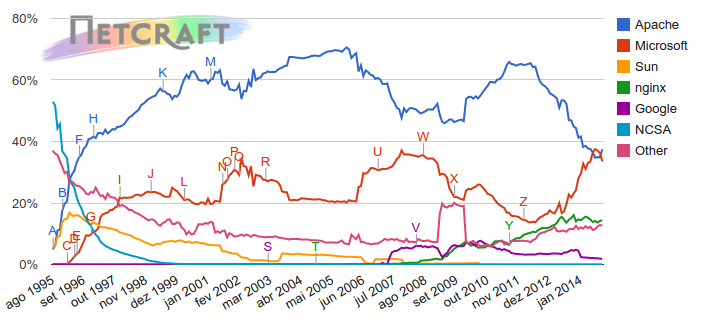
\includegraphics[width=1\linewidth]{../figuras/grafico1}\\
		Fonte: Netcraft
	\end{figure}
\end{frame}
% ----------------- SLIDE 7 --------------------------------
\begin{frame}{Utilização dos Servidores \textit{Web}}
	\begin{figure}
		\centering
		\caption{Utilização de Servidores \textit{web} entre os 1.000.000 de 
		sítios 
		}
		mais acessados no mundo.
		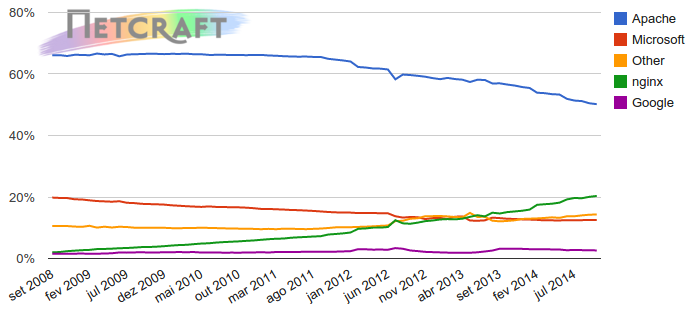
\includegraphics[width=1\linewidth]{../figuras/grafico2} \\
		Fonte: Netcraft
	\end{figure}
\end{frame}
% ----------------- SLIDE 8 --------------------------------
\begin{frame}{Utilização dos Servidores \textit{Web}}
	\begin{itemize}
		\item Queda na utilização do Apache; \pause
		\item Aumento da utilização do Nginx; \pause
		\item Tecnologia em ascensão não significar ser melhor; \pause
		\item Investigar é necessário.
	\end{itemize}
\end{frame}

\subsection*{Motivação}
% ----------------- SLIDE 9 --------------------------------
\begin{frame}{Motivação}
	\begin{itemize}
		\item Aumento do número de usuários; \pause
		\item Lentidão eventual do sistema; \pause
		\item 3.500 novos alunos por ano.
	\end{itemize}
\end{frame}
% ----------------- SLIDE 10 --------------------------------
\begin{frame}{Motivação}
	\framesubtitle{Pessoas ligadas à UFVJM}
	\centering
	\begin{table}
		\caption{Pessoas ligadas à UFVJM}
		\begin{tabular}{|c|c|}
			\hline
			Alunos & 8.121 \\ \hline
			Professores & 576 \\ \hline
			Servidores Técnico-Administrativo & 421 \\ \hline
			\textbf{Total} & 9.118 \\ \hline
		\end{tabular}
	\end{table}
	Fonte: UFVJM Em Números
\end{frame}
% ----------------- SLIDE 11 --------------------------------
\begin{frame}{Motivação}
	\framesubtitle{Dez dias com mais acessos ao SIGA}
	\centering
	{\small \begin{table}
		\caption{Dez dias com mais acessos no SIGA}
		\begin{tabular}{|c|c|c|}
			\hline
			\textbf{Dia} & \textbf{Acessos}  & \textbf{Ocasião} \\ \hline
			16/08/2014 & 20.942 & Início da Pré Matrícula \\ \hline
			25/08/2014 & 17.536 & Início do Período Letivo \\ \hline
			16/04/2013 & 17.091 & Dias Finais do Período Letivo \\ \hline
			30/09/2013 & 17.007 & Início da Pré Matrícula \\ \hline
			17/04/2013 & 16.772 & Dias Finais do Período Letivo \\ \hline
			15/04/2013 & 16.597 & Dias Finais do Período Letivo \\ \hline
			31/07/2014 & 16.035 & Dias Finais do Período Letivo \\ \hline
			29/07/2014 & 15.744 & Dias Finais do Período Letivo \\ \hline
			28/07/2014 & 15.477 & Dias Finais do Período Letivo \\ \hline
			30/07/2014 & 14.854 & Dias Finais do Período Letivo \\ \hline
		\end{tabular}
	\end{table}}
	Fonte: Base de Dados do SIGA
\end{frame}

\subsection*{Objetivos}
% ----------------- SLIDE 12 --------------------------------
\begin{frame}{Objetivos}
	\begin{block}{Objetivo Geral}
		Identificar se a utilização do servidor HTTP Nginx é mais eficiente do 
		que o utilizado atualmente, o Apache HTTP \textit{Server}.
	\end{block} \pause
	\begin{block}{Objetivos Específicos}
		Analisar os dados coletados a partir de testes realizados para 
		identificar se o Nginx é mais eficiente do que o Apache; apresentar a 
		solução encontrada e analisar o que pode ser feito para evitar a 
		substituição ou reconstrução do SIGA.
	\end{block}
\end{frame}